\documentclass[25pt, a0paper, portrait, margin=0mm, innermargin=15mm, blockverticalspace=15mm,
  colspace=15mm, subcolspace=8mm]{tikzposter}
\usepackage[default]{lato}
\usepackage{booktabs}
\usepackage{array}
\newcolumntype{L}[1]{>{\raggedright\arraybackslash}p{#1}}
\usepackage{qrcode}
\usetikzlibrary{positioning,arrows.meta}

% Vulkanised 2027's colours; its header art comes from `make art`, plain red without it.
\definecolor{vkred}{HTML}{A71C33}
\definecolor{vkdark}{HTML}{1B1B1B}
\definecolor{vklight}{HTML}{F6F6F6}
\definecolorstyle{Vulkanised}{
  \colorlet{colorOne}{vkred}\colorlet{colorTwo}{vkdark}\colorlet{colorThree}{vklight}
}{
  \colorlet{backgroundcolor}{white}\colorlet{framecolor}{white}
  \colorlet{titlefgcolor}{white}\colorlet{titlebgcolor}{vkred}
  \colorlet{blocktitlebgcolor}{vkred}\colorlet{blocktitlefgcolor}{white}
  \colorlet{blockbodybgcolor}{vklight}\colorlet{blockbodyfgcolor}{vkdark}
  \colorlet{innerblocktitlebgcolor}{white}\colorlet{innerblocktitlefgcolor}{vkdark}
  \colorlet{innerblockbodybgcolor}{white}\colorlet{innerblockbodyfgcolor}{vkdark}
  \colorlet{notefgcolor}{vkdark}\colorlet{notebgcolor}{white}\colorlet{noteframecolor}{vkred}
}
\definetitlestyle{Lava}{width=\paperwidth, roundedcorners=0, linewidth=0pt, innersep=7cm,
  titletotopverticalspace=0mm, titletoblockverticalspace=15mm}{
  \begin{scope}
    \clip (\titleposleft, \titleposbottom) rectangle (\titleposright, \titlepostop);
    \fill[vkred] (\titleposleft, \titleposbottom) rectangle (\titleposright, \titlepostop);
    \IfFileExists{build/art/header.jpg}{\node[anchor=south west, inner sep=0] at (\titleposleft, \titleposbottom)
      {\includegraphics[width=\paperwidth]{build/art/header.jpg}};}{}
    \fill[black, opacity=0.5] (\titleposleft, \titleposbottom) rectangle (\titleposright, \titlepostop);
  \end{scope}}
\usetheme{Simple}
\useblockstyle{Default}
\usetitlestyle{Lava}
\makeatletter
\renewcommand{\TP@maketitle}{\centering\color{titlefgcolor}{\bfseries\Huge\@title\par}\vspace*{1.2em}
  {\huge\@author\par}\vspace*{0.5em}{\LARGE\@institute}}
\makeatother
\tikzposterlatexaffectionproofoff
\usecolorstyle{Vulkanised}
\newcommand{\photo}[1]{\fbox{\parbox[c][17cm]{0.9\linewidth}{\centering\textit{photo: #1}}}}

\title{Borg: Vulkan from vkcube Down to the Gates}
\author{Andreas Wendleder}
\institute{Independent researcher \quad github.com/gonsolo/Borg \quad Vulkanised 2027, Kortrijk}

\begin{document}
\maketitle

\block{}{
  \begin{minipage}[c]{0.5\linewidth}
    \Large An open-source GPU small enough for one person to read end to end: about 11,000 lines of
    Chisel, a 64-bit RISC-V CPU around it that boots Linux, and a native Mesa Vulkan driver in Rust
    with its own shader compiler. The unmodified Khronos \texttt{cube.c} renders on an FPGA, and the
    Vulkan CTS runs on the FPGA itself, checked against a simulator of the RTL.
  \end{minipage}\hfill
  \begin{minipage}[c]{0.46\linewidth}
    \centering\photo{the Nexys Video, vkcube full screen over HDMI}\\[3mm]
    \normalsize The unmodified \texttt{cube.c} under Linux on Hutt, on a Nexys Video (Artix-7).
  \end{minipage}
}

\begin{columns}
\column{0.333}
\block{One driver, three back ends}{
  \centering
  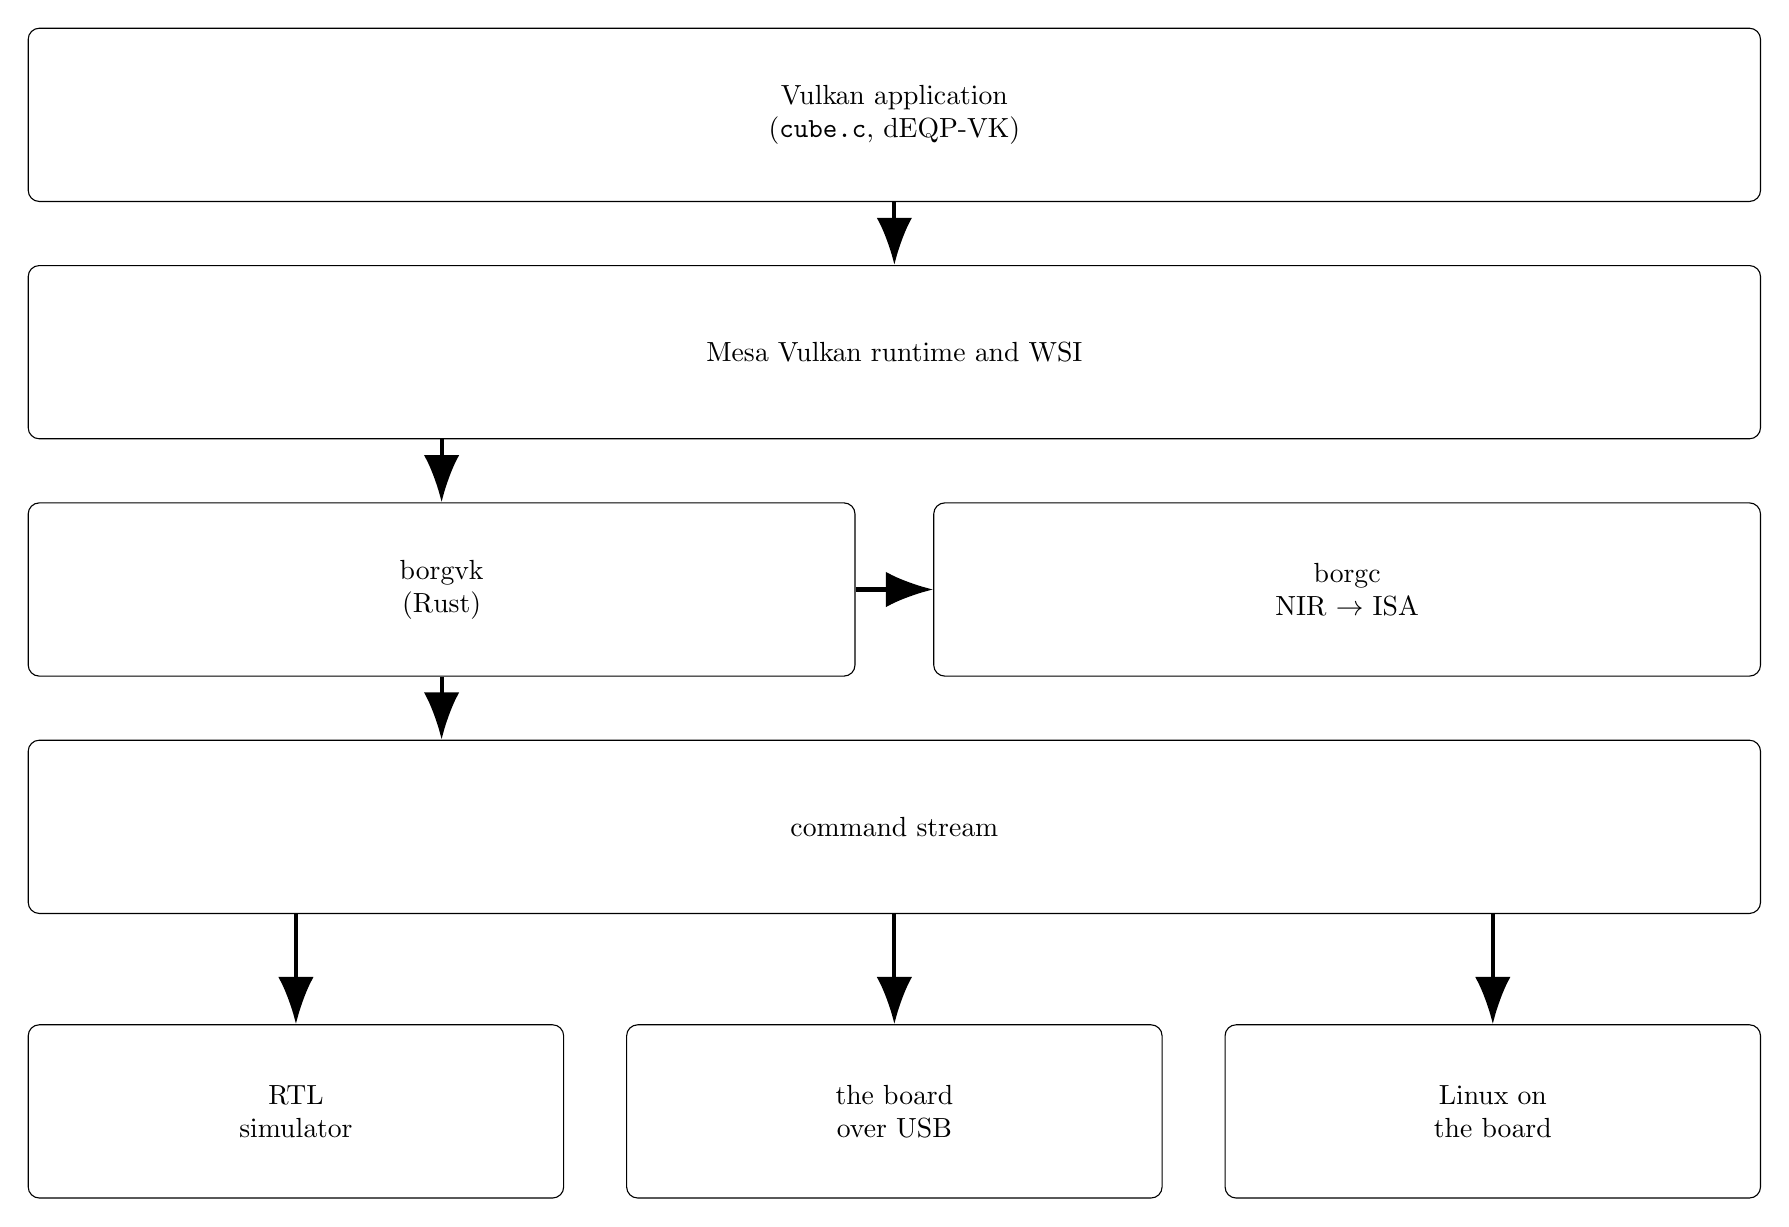
\begin{tikzpicture}[box/.style={draw, rounded corners=4pt, align=center, minimum height=22mm,
      inner sep=8pt, fill=white}, arr/.style={-{Latex[length=6mm]}, line width=1.5pt}]
    \node[box, minimum width=22cm] (app) {Vulkan application\\(\texttt{cube.c}, dEQP-VK)};
    \node[box, minimum width=22cm, below=8mm of app] (rt) {Mesa Vulkan runtime and WSI};
    \node[box, minimum width=10.5cm, below=8mm of rt.south west, anchor=north west] (vk) {borgvk\\(Rust)};
    \node[box, minimum width=10.5cm, below=8mm of rt.south east, anchor=north east] (cc) {borgc\\NIR $\to$ ISA};
    \node[box, minimum width=22cm, below=8mm of vk.south west, anchor=north west] (pk) {command stream};
    \node[box, below=14mm of pk.south west, anchor=north west, minimum width=6.8cm] (sim) {RTL\\simulator};
    \node[box, below=14mm of pk.south, minimum width=6.8cm] (usb) {the board\\over USB};
    \node[box, below=14mm of pk.south east, anchor=north east, minimum width=6.8cm] (lin) {Linux on\\the board};
    \draw[arr] (app) -- (rt); \draw[arr] (rt.south -| vk) -- (vk); \draw[arr] (vk) -- (cc);
    \draw[arr] (vk.south) -- (vk.south |- pk.north);
    \draw[arr] (pk.south -| sim) -- (sim); \draw[arr] (pk) -- (usb); \draw[arr] (pk.south -| lin) -- (lin);
  \end{tikzpicture}\\[8mm]
  \raggedright
  The same driver code in every case. The simulator is for bring-up and debugging, the board over
  USB runs the conformance suite, and under Linux a Rust DRM driver takes the stream.
}
\block{One device heap, every target}{
  One heap at the same GPU address on every back end: buffers, images and render targets are used
  in place. How it stays in sync:
  \begin{center}
  \begin{tabular}{L{0.25\linewidth}L{0.34\linewidth}L{0.34\linewidth}}
    \toprule
    & CPU writes reach Borg & Borg's writes reach the CPU \\
    \midrule
    Simulator & shared memory & shared memory \\
    Board over USB & changed pages, before a job & dirty pages from a bitmap, after it \\
    Linux & GEM objects at their GPU address & write-through cache, flushed on Borg's writes \\
    \bottomrule
  \end{tabular}
  \end{center}
}

\column{0.333}
\block{What Vulkan 1.0 asks of hardware}{
  \begin{tabular}{L{0.42\linewidth}L{0.52\linewidth}}
    \toprule
    Requirement & Borg mechanism \\
    \midrule
    Compute on every graphics queue & workgroups on the shader core, barrier, atomics \\
    Derivatives, implicit LOD & 2x2 quad on four lanes \\
    Sampled images, samplers & descriptor-table texture unit, 51 formats, mipmaps \\
    Colour attachment formats & raw attachments, blending by read-back \\
    Depth, stencil, blend & fixed function per tile \\
    Occlusion queries & exact sample counts \\
    4x MSAA & passes per tile \\
    Vertex input, topologies & hardware draw front end, homogeneous setup \\
    \bottomrule
  \end{tabular}
}
\block{A compiler for 32 registers}{
  The ISA is a RISC-V subset (RV32I, Zfinx, Zmmul, Zicond) with the GPU instructions in the custom
  opcode space. One opcode file, in the format of \texttt{riscv-opcodes}, generates the hardware
  decoder, the C header and the compiler's encoder:\\[5mm]
  {\ttfamily fmadd.s rd rs1 rs2 rs3 rm 26..25=0 6..2=0x10\\
  texd \ \ \ rd rs1 rs2 rs3 26..25=0 6..2=0x0A}\\[5mm]
  borgc refuses what it cannot compile instead of guessing. Work a fragment shader does from push
  constants alone moves into the vertex shader, once per triangle:
  \begin{center}
  \begin{tabular}{lrr}
    \toprule
    Instructions & per pixel & per triangle \\
    \midrule
    before & 320 & 87 \\
    after & 133 & 281 \\
    \bottomrule
  \end{tabular}
  \end{center}
}

\column{0.333}
\block{The CTS against the hardware}{
  \textbf{Simulator first.} The GPU's RTL compiled with CIRCT's arcilator, about 120,000 cycles per
  second: every signal visible.\\[4mm]
  \textbf{Then the board.} The same command stream over USB to the Nexys Video: Borg at 25 MHz, the
  link at about 15 MB/s. Board and simulator agree byte for byte on 825 recorded driver cases.\\[4mm]
  A quick list of 114 cases runs in 16 s. The slowest known cases pass on the board in five
  minutes to an hour.
  \begin{center}\fbox{\parbox[c][13cm]{0.9\linewidth}{\centering\textit{results by group,
  from the clean full run on the board}}}\end{center}
}
\block{Found before silicon}{
  \begin{itemize}
    \item \texttt{textureGather}: one subtap instead of the average at cube corners.
    \item Integer bits through a float move, flushed as denormals.
    \item Branch targets one word early.
    \item A constant built after the instructions that read it.
    \item A simulator read that gave up early: slow cases passed with half-drawn images.
  \end{itemize}
}
\end{columns}

\block{Lessons for a new implementation}{
  \begin{minipage}[c]{0.68\linewidth}
    \begin{itemize}
      \item Bring up the \texttt{api} group first, and compute early.
      \item Get onto an FPGA early; check it byte for byte against the simulator.
      \item Refuse what the compiler cannot do; keep one source of truth for the ISA.
      \item Distrust a pass that comes too fast.
    \end{itemize}
  \end{minipage}\hfill
  \begin{minipage}[c]{0.3\linewidth}
    \centering
    \qrcode[height=6cm]{https://github.com/gonsolo/Borg}\hspace{1.5cm}\qrcode[height=6cm]{https://gonsolo.github.io/Borg/}\\[3mm]
    \small code \hspace{5.5cm} book
  \end{minipage}
}
\end{document}
